\section{Auswertung}
\label{sec:auswertung}
\subsection{Statische Methode}
\label{sec:as}

\begin{figure}[H]
    \centering
    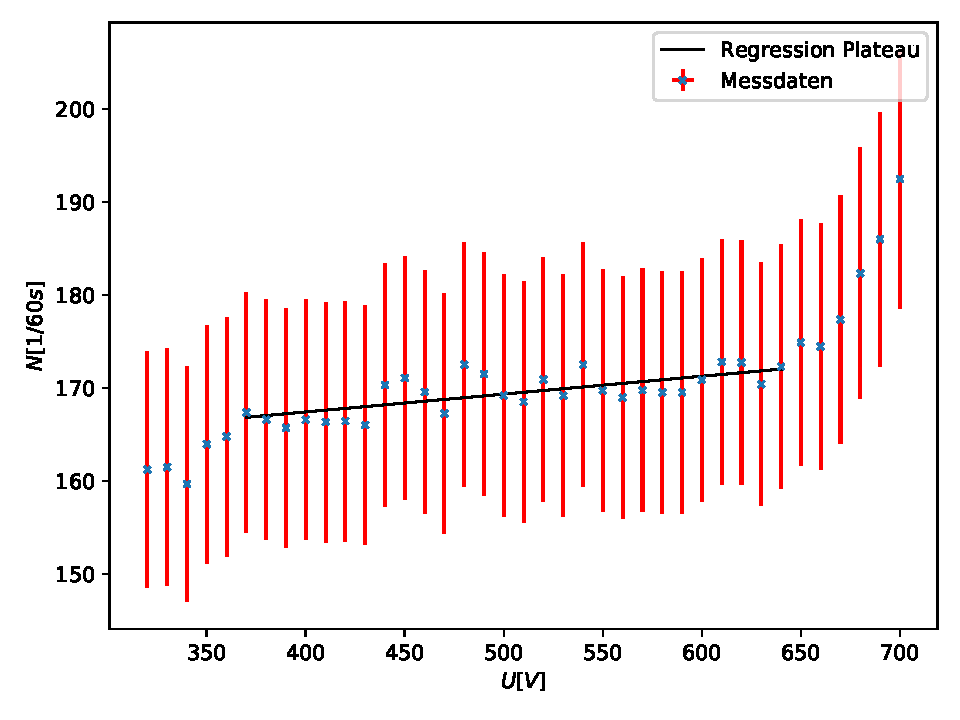
\includegraphics[width=\textwidth]{build/plot1.pdf}
    \caption{Temperaturverlauf der fernen Thermoelemente.}
    \label{fig:messing}
\end{figure}
\noindent

\begin{figure}[H]
    \centering
    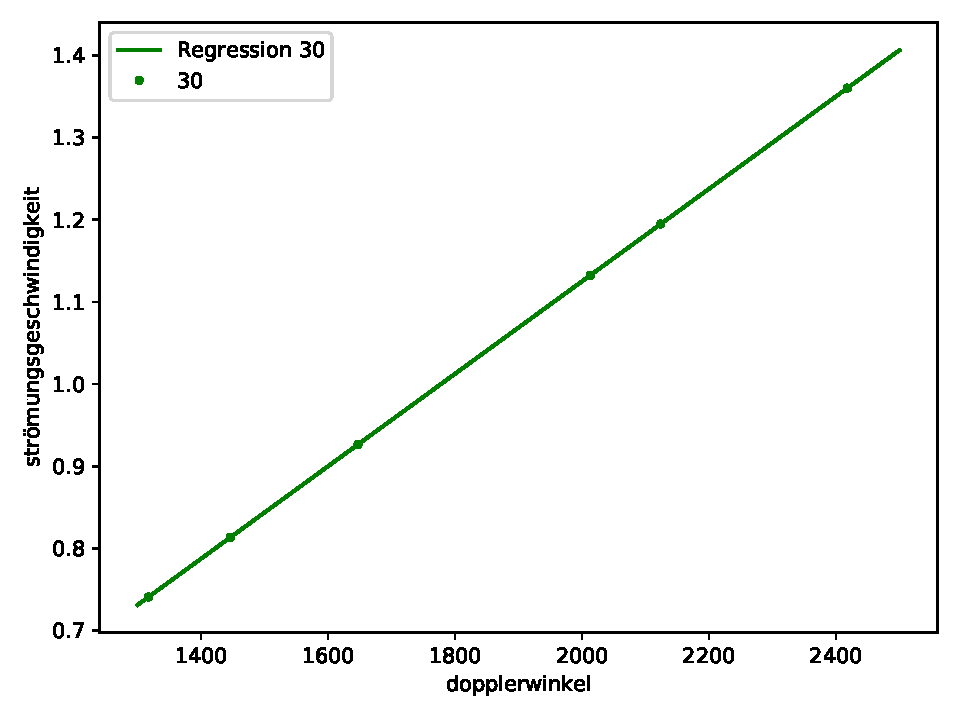
\includegraphics[width=\textwidth]{build/plot2.pdf}
    \caption{Temperaturdifferenz $T_{St}$ zwischen dem breiten Messingstab und dem Edelstahlstab.}
    \label{fig:temp}
\end{figure}
\noindent

\subsection{Dynamische Methode}
\label{sec:ad}
In Abbildung \ref{fig:messing} sind die Temperaturverläufe des breiteren Messingstabes graphisch aufgetragen. Dabei wurde der Stab nach Kapitel
\ref{sec:durchführung} mit einer Periodendauer von $\SI{80}{\second}$ geheizt.

\begin{figure}[H]
    \centering
    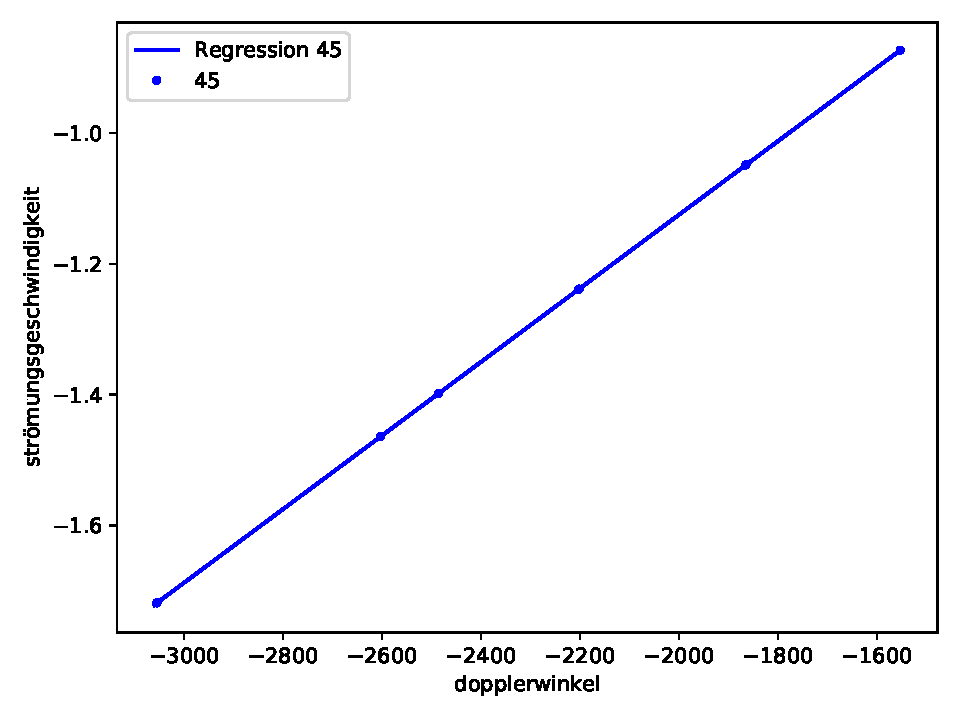
\includegraphics[width=\textwidth]{build/plot3.pdf}
    \caption{Temperaturverläufe des breiteren Messingstabes mit einer Periodendauer von $\SI{80}{\second}$.}
    \label{fig:messing}
\end{figure}
\noindent

Aus dem Graphen werden durch ablesen die Amplituden $A_{nah}$ und $A_{fern}$ und die Phasenverschiebung $\delta t$ zwischen $T_{nah}$ und 
$T_{fern}$ bestimmt. Diese abgelesenen Werte sind in Tabelle \ref{tab:messing}  aufgelistet. 

\begin{table}[H]                                                                                   
    \centering                                                                                     
        \caption{Amplituden $A$ und Phasenverschiebung $\Delta t$ von Messing.}                      
        \label{tab:messing}                                                                        
        \sisetup{table-format=1.2}                                                                 
        \begin{tabular}{S S S[table-format=2.0] S[table-format=3.2]}                                                   
          \toprule                                                                                 
          {$A_{nah}[\si{\kelvin}]$} & {$A_{fern}[\si{\degree}]$} & {$\delta t[\si{\second}]$} & {$\kappa [\si{\watt\per\milli\kelvin}]$}\\                                            
          \midrule                                                                                 
           0.00 & 0.00 & 00 & 000.00 \\
          \bottomrule                                                                              
        \end{tabular}                                                                              
      \end{table}
\noindent                                             

Vollkommen analog sind in Abbildung \ref{fig:alu} die Temperaturverläufe für Aluminium dargestellt. Die abgelesenen Werte finden sich in 
Tabelle \ref{tab:alu}. 

\begin{figure}[H]
    \centering
    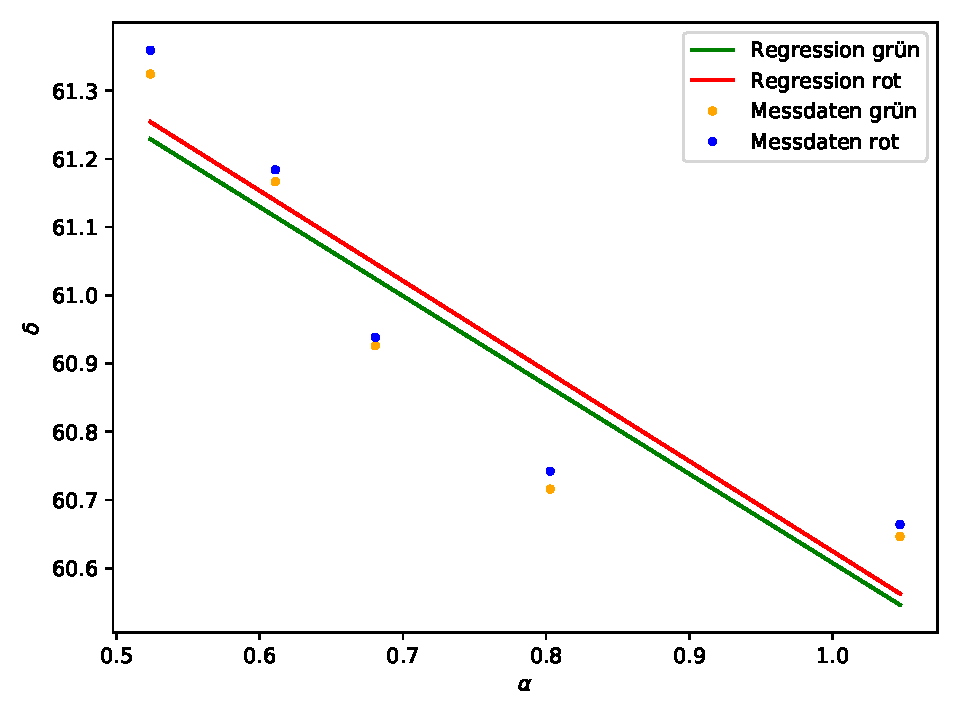
\includegraphics[width=\textwidth]{build/plot4.pdf}
    \caption{Temperaturverläufe des Aluminiumstabes mit einer Periodendauer von $\SI{80}{\second}$.}
    \label{fig:alu}
\end{figure}
\noindent

\begin{table}[H]                                                                                   
    \centering                                                                                     
        \caption{Amplituden $A$ und Phasenverschiebung $\Delta t$ von Aluminium.}                      
        \label{tab:alu}                                                                        
        \sisetup{table-format=1.2}                                                                 
        \begin{tabular}{S S S[table-format=2.0] S[table-format=3.2]}                                                   
          \toprule                                                                                 
          {$A_{nah}[\si{\kelvin}]$} & {$A_{fern}[\si{\degree}]$} & {$\delta t[\si{\second}]$} & {$\kappa [\si{\watt\per\milli\kelvin}]$}\\                                            
          \midrule                                                                                 
           0.00 & 0.00 & 00 & 000.00 \\
          \bottomrule                                                                              
        \end{tabular}                                                                              
      \end{table}     
\noindent



\begin{figure}[H]
    \centering
    \includegraphics[width=\textwidth]{build/plot5.pdf}
    \caption{Temperaturverläufe des Edelstahlstabes mit einer Periodendauer von $\SI{200}{\second}$.}
    \label{fig:stahl}
\end{figure}
\noindent

\begin{table}[H]                                                                                   
    \centering                                                                                     
        \caption{Amplituden $A$ und Phasenverschiebung $\Delta t$ von Edelstahl.}                      
        \label{tab:stahl}                                                                        
        \sisetup{table-format=1.2}                                                                 
        \begin{tabular}{S S S[table-format=2.0] S[table-format=3.2]}                                                   
          \toprule                                                                                 
          {$A_{nah}[\si{\kelvin}]$} & {$A_{fern}[\si{\degree}]$} & {$\delta t[\si{\second}]$} & {$\kappa [\si{\watt\per\milli\kelvin}]$}\\                                            
          \midrule                                                                                 
           0.00 & 0.00 & 00 & 000.00 \\
          \bottomrule                                                                              
        \end{tabular}                                                                              
      \end{table}     
\noindent